\documentclass[oneside,a4paper,openany,11pt]{ctexbook}

\usepackage{geometry}
\geometry{          %% 调整页边距
    verbose,        % 提示信息
    a4paper,        % 纸张大小
    left=2.0cm,     % 左边距
    right=2.0cm,    % 右边距
    top=2.5cm,      % 上边距
    bottom=2.2cm    % 下边距
}


\usepackage{amsmath,amssymb,amsfonts,amsthm}
\newcommand*{\dif}{\mathop{}\!\mathrm{d}} % 定义微分算子


\usepackage{graphicx}


\ctexset{%
    section/format += \raggedright
}


\usepackage[version=4]{mhchem}
\usepackage{siunitx}
% \usepackage{tikz}


\usepackage{makeidx} % 调用 makeidx 宏包,用来处理索引
\makeindex % 开启索引的收集
\bibliographystyle{plain} % 指定参考文献样式为 plain


\usepackage[breaklinks,colorlinks,linkcolor=black,citecolor=black,urlcolor=black]{hyperref}
%%%%% url自动断词换行 %%%%%
\makeatletter
\def\UrlAlphabet{%
      \do\a\do\b\do\c\do\d\do\e\do\f\do\g\do\h\do\i\do\j%
      \do\k\do\l\do\m\do\n\do\o\do\p\do\q\do\r\do\s\do\t%
      \do\u\do\v\do\w\do\x\do\y\do\z\do\A\do\B\do\C\do\D%
      \do\E\do\F\do\G\do\H\do\I\do\J\do\K\do\L\do\M\do\N%
      \do\O\do\P\do\Q\do\R\do\S\do\T\do\U\do\V\do\W\do\X%
      \do\Y\do\Z}
\def\UrlDigits{\do\1\do\2\do\3\do\4\do\5\do\6\do\7\do\8\do\9\do\0}
\g@addto@macro{\UrlBreaks}{\UrlOrds}
\g@addto@macro{\UrlBreaks}{\UrlAlphabet}
\g@addto@macro{\UrlBreaks}{\UrlDigits}
\makeatother
%%%%% url自动断词换行 %%%%%


\title{《固体物理学》习题解答}
\author{祝茗}
\date{\today}

\begin{document}

\frontmatter
\maketitle
\chapter{前言\label{ch:preface}}

本文前身为,华中师范大学物理科学与技术学院 2003 级师生于 2006 年 6 月编撰的《固体物理学》学习解答。

\begin{figure}[htbp]
    \centering
    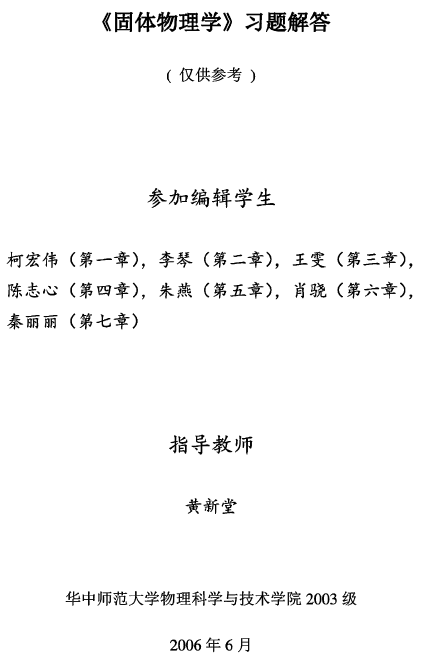
\includegraphics[width=0.6\textwidth]{pic/原封面页.png}
    \caption{原封面页}
\end{figure}

本文使用 \LaTeX{} 重排,旨在改正一些笔误的同时,翻新答案,为大家提供便利。

若有错误眼拙未能修正,还望见谅。

\tableofcontents

\mainmatter
\chapter{晶体结构\label{ch:1}}

\noindent \textbf{1.\quad} 氯化钠与金刚石型结构是复式格子还是布拉维格子,各自的基元为何?写出这两种结构的原胞与晶胞基矢,设晶格常数为 $a$。

\noindent \textbf{解:}

氯化钠与金刚石型结构都是复式格子。氯化钠的基元为一个 \ce{Na} 用和一个 \ce{Cl} 一组成的正负离子对。金刚石的基元是一个面心立方上的 \ce{C} 原子和一个体对角线上的 \ce{C} 原子组成的 \ce{C} 原子对。

由于 \ce{NaCl} 和金刚石都由面心立方结构套构而成,所以,其\emph{元胞基矢}都为:

\begin{equation*}
    \begin{cases}
        \mathbf{a}_1 = \frac{a}{2} (\mathbf{j} + \mathbf{k}) \\
        \mathbf{a}_2 = \frac{a}{2} (\mathbf{k} + \mathbf{i}) \\
        \mathbf{a}_3 = \frac{a}{2} (\mathbf{i} + \mathbf{j})
    \end{cases}
\end{equation*}

相应的\emph{晶胞基矢}都为:

\begin{equation*}
    \begin{cases}
        \mathbf{a} = a \mathbf{i} \\
        \mathbf{b} = b \mathbf{j} \\
        \mathbf{c} = c \mathbf{k}
    \end{cases}
\end{equation*}

\noindent \textbf{2.\quad} 六角密集结构可取四个原胞基矢 $\mathbf{a}_1, \mathbf{a}_2, \mathbf{a}_3$ 与 $\mathbf{c}$,如图所示。

\begin{figure}[htbp]
    \centering
    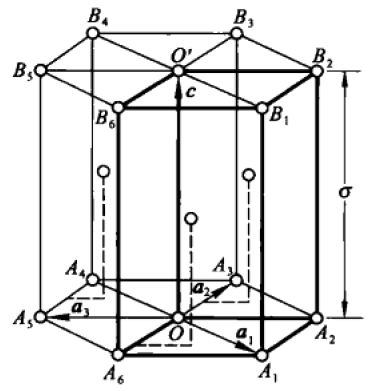
\includegraphics{pic/六方.png}
    \caption{六方}
    \label{fig:1.1}
\end{figure}

\noindent 试写出 $O^\prime A_1 A_3$、$A_1 A_3 B_3 B_1$、$A_2 B_2 B_5 A_5$、$A_1 A_2 A_3 A_4 A_5 A_6$ 这四个面所属晶面族的晶面指数 $(h\ k\ l\ m)$。

\noindent \textbf{解:}

\begin{enumerate}
    \item 对于 $O^\prime A_1 A_3$ 面,其在四个原胞基矢上的截矩分别为:$1, 1, -\frac{1}{2}, 1$。所以,其晶面指数为 $(11\bar{2}1)$。
    \item 对于 $A_1 A_3 B_3 B_1$ 面,其在四个原胞基矢上的截矩分别为:$1, 1, -\frac{1}{2}, \infty$。所以,其晶面指数为 $(11\bar{2}0)$ 。
    \item 对于 $A_2 B_2 B_5 A_5$ 面,其在四个原胞基矢上的截矩分别为:$1, -1, \infty, \infty$。所以,其晶面指数为 $(1\bar{1}00)$。
    \item 对于 $A_1 A_2 A_3 A_4 A_5 A_6$ 面,其在四个原胞基矢上的截矩分别为:$\infty, \infty, \infty, 1$。所以,其晶面指数为 $(0001)$。
\end{enumerate}

\noindent \textbf{3.\quad} 如将等体积的硬球堆成下列结构,求证球体可能占据的最大体积与总体积的比为:简立方:$\frac{\pi}{6}$;体心立方:$\frac{\sqrt{3}\pi}{8}$;面心立方:$\frac{\sqrt{2}\pi}{6}$;六角密集:$\frac{\sqrt{2}\pi}{6}$;金刚石:$\frac{\sqrt{3}\pi}{16}$;

\noindent \textbf{证明:}

由于晶格常数为 $a$, 所以:

构成简立方时,最大球半径为 $R_m=\frac{a}{2}$,每个原胞中占有一个原子,

\begin{align*}
    \therefore V_m &= \frac{4}{3} \pi \left(\frac{a}{2}\right)^3 = \frac{\pi}{6} a^3 \\
    \therefore \frac{V_m}{a^3} &= \frac{\pi}{6}
\end{align*}

构成体心立方时,体对角线等于 $4$ 倍的最大球半径,即:$4 R_m=\sqrt{3} a$,每个晶胞中占有两个原子,

\begin{align*}
    \therefore 2 V_m &= 2 \times \frac{4}{3} \pi \left(\frac{\sqrt{3}}{4} a\right)^3 = \frac{\sqrt{3}\pi}{8} a^3 \\
    \therefore \frac{2 V_m}{a^3} &= \frac{\sqrt{3}\pi}{8}
\end{align*}

构成面心立方时,面对角线等于 $4$ 倍的最大球半径,即:$4 R_m=\sqrt{2}a$ 正每个晶胞占有 $4$ 个原子,

\begin{align*}
    \therefore 4 V_m &= 4 \times \frac{4}{3} \pi \left(\frac{\sqrt{2}}{4} a\right)^3 = \frac{\sqrt{2}\pi}{6} a^3 \\
    \therefore \frac{4 V_m}{a^3} &= \frac{\sqrt{2}\pi}{6}
\end{align*}

构成六角密集结构时,中间层的三个原子与底面中心的那个原子恰构成一个正四面体,其高则正好是其原胞基矢 $c$ 的长度的一半,由几何知识易知 $|c|=-R_m$。原胞底面边长为 $2 R_m$。每个晶胞占有两个原子,

\begin{equation*}
    \therefore 2 V_m = 2 \times \frac{4}{3} \pi R_m^3 = \frac{8}{3} \pi R_m^3
\end{equation*}

原胞的体积为:$V=(2 R_m)^2 \sin \ang{60} \cdot \frac{4\sqrt{6}}{3} R_m = 8\sqrt{2} R_m^3$

\begin{equation*}
    \therefore \frac{2 V_m}{V} = \frac{\pi}{3\sqrt{2}} = \frac{\sqrt{2}\pi}{6}
\end{equation*}

构成金刚石结构时,一的体对角线长度等于两个最大球半径,即:$2 R_m=\frac{\sqrt{3}}{4} a$,每个晶胞包含 $8$ 个原子,

\begin{align*}
    \therefore 8 V_m &= 8 \times \frac{4}{3} \pi \left(\frac{\sqrt{3}}{8} a\right)^3 = \frac{\sqrt{3}\pi}{16} a^3 \\
    \therefore \frac{8 V_m}{a^3} &= \frac{\sqrt{3}\pi}{16}
\end{align*}

\noindent \textbf{4.\quad} 金刚石结构原子间的键间角与立方体的体对角线间的夹角相同,试用矢量分析的方法证明这一夹角为 \ang{109;28}。

\noindent \textbf{证明:}

如图所示,沿品胞基矢的方向建立坐标系,并设晶格常数为 $1$。选择体对角线 $\overline{AB}$ 和 $\overline{CD}$,用坐标表示为 $\{1, 1, -1\}$ 和 $\{-1, 1, 1\}$。

\begin{figure}[htbp]
    \centering
    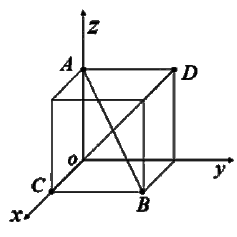
\includegraphics{pic/坐标系1.png}
    \caption{沿品胞基矢的方向建立坐标系。}
    \label{fig:1.2}
\end{figure}

所以,其夹角的余弦为:

\begin{align*}
    \cos\theta &= \frac{\overline{AB} \cdot \overline{CD}}{|\overline{AB}| \cdot |\overline{CD}|} \\
    \therefore \theta &= \arccos\left(-\frac{1}{3}\right) = \ang{109;28}
\end{align*}

\noindent \textbf{5.\quad} 试求面心立方结构 $(110)$ 和 $(111)$ 晶面族的原子数面密度,设晶格常数为 $a$。

\noindent \textbf{解:}

\begin{figure}[htbp]
    \centering
    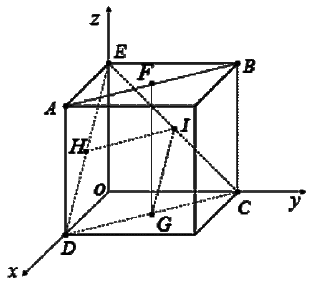
\includegraphics{pic/坐标系2.png}
    \caption{}
    \label{fig:1.3}
\end{figure}

如图所示,面 $ABCD$ 即 $(110)$ 面,面 $COE$ 即为 $(111)$ 面。设该面心立方的晶格常数为 $a$, 则在 $(110)$ 面内选取只包含一个原子的面 $AFGD$,其面积为 $a \cdot \frac{\sqrt{2}}{2} a=\frac{\sqrt{2}}{2} a^2$,所以其原子数面密度为

\begin{equation*}
    \frac{1}{\frac{\sqrt{2}}{2} a^2} = \frac{\sqrt{2}}{a^2}
\end{equation*}

在 $(111)$ 面内选取只包含一个原子的面 $DHIG$,其面积为:$\left(\frac{\sqrt{2}}{2}a\right)^2 \sin \frac{\pi}{3}=\frac{\sqrt{3}}{4} a^2$ 所以其原子数面密度为:

\begin{equation*}
    \frac{1}{\frac{\sqrt{3}}{4} a^2} = \frac{4\sqrt{3}}{3} a^2
\end{equation*}

\noindent \textbf{6.\quad} 若在面心立方结构的立方体心位置上也有一原子,试确定此结构的原胞,每个原胞内包含几个原子,设立方边长为 $a$。

\noindent \textbf{解:}

这种体心立方结构中有五种不同的原子。顶角、体心上的原子是两种不同的原子,另外,面心上的原子前后、上下、左右的原子两两一组,是互不相同的原子。故此种结构共有五种不同的原子,整个面心立方就是一个原胞。每个原胞中的原子数为:

\begin{equation*}
    8 \times \frac{1}{8} + 1 + 3 \times 2\times \frac{1}{2} = 5 (\text{个})
\end{equation*}

\noindent \textbf{7.\quad} 底心立方 (立方顶角与上、下底心处有原子)、侧心立方 (立方顶角与四个侧面的中心处有原子) 与边心立方 (立方顶角与十二条棱的中点有原子) 各属何种布拉维格子?每个原胞包含几个原子?

\noindent \textbf{解:}

这三种结构都属于简立方结构,原胞包含的原子数分别为:

\begin{enumerate}
    \item 底心立方:$\frac{1}{8} \times 8 = 1$
    \item 侧心立方:$\frac{1}{8} \times 8 + \frac{1}{2} \times 4 = 3$
    \item 边心立方:$\frac{1}{8} \times 8 + \frac{1}{4} \times 12 = 4$
\end{enumerate}

\noindent \textbf{8.\quad} 试证六角密集结构 $\frac{c}{a}=\sqrt{\frac{8}{3}}\approx 1.63$

\begin{figure}[htbp]
    \centering
    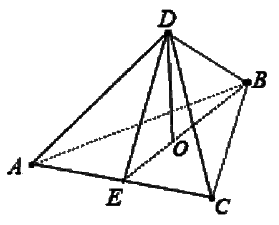
\includegraphics{pic/正四面体.png}
    \caption{正四面体}
    \label{fig:1.4}
\end{figure}

如图所示,$ABC$ 分别表示六角密集结构中中间层的三个原子,$D$ 表示底面中心的原子。$DABC$ 构成一个正四面体,为长为 $a$

$DO \perp \text{面} ABC$,则 $|DO|=\frac{c}{2}$

\begin{equation*}
    \because DE = \frac{\sqrt{3}}{2} a, \quad OE = \frac{1}{3} \cdot \frac{\sqrt{3}}{2} a = \frac{\sqrt{3}}{6} a
\end{equation*}

且 $DO \perp OE$,则由勾股定理可得

\begin{equation*}
    OD = \sqrt{\left(\frac{\sqrt{3}}{2}a\right)^2-\left(\frac{\sqrt{6}}{3}a\right)^2} = \frac{\sqrt{6}}{3} a
\end{equation*}

\begin{equation*}
    \therefore c = 2 OD = \frac{2\sqrt{6}}{3} a, \quad \frac{c}{a} = \frac{2\sqrt{6}}{3} = \sqrt{\frac{8}{3}} \approx 1.63
\end{equation*}

\chapter{晶体中的衍射\label{ch:2}}

\noindent \textbf{1.\quad} 试证明面心立方与体心立方互为正倒格子。

\noindent \textbf{方法1:}

面心立方:

\begin{align*}
    a_1 &= \frac{a}{2} (\vec{j}+\vec{k}) \\
    a_2 &= \frac{a}{2} (\vec{k}+\vec{i}) \\
    a_3 &= \frac{a}{2} (\vec{i}+\vec{j})
\end{align*}

由正格子和倒格子的转换关系

\begin{align*}
    \vec{b}_1 &= 2\pi (\vec{a}_2 \times \vec{a}_3) / \Omega \\
    \vec{b}_2 &= 2\pi (\vec{a}_3 \times \vec{a}_1) / \Omega \\
    \vec{b}_3 &= 2\pi (\vec{a}_1 \times \vec{a}_2) / \Omega
\end{align*}

其中 $\Omega=\vec{a}_1 \cdot (\vec{a}_2 \times \vec{a}_3)$,计算可得

\begin{align*}
    \vec{b}_1 &= \frac{2\pi}{a} (-\vec{i}+\vec{j}+\vec{k}) / \Omega \\
    \vec{b}_2 &= \frac{2\pi}{a} (\vec{i}-\vec{j}+\vec{k}) / \Omega \\
    \vec{b}_3 &= \frac{2\pi}{a} (\vec{i}+\vec{j}-\vec{k}) / \Omega
\end{align*}

在体心立方中

\begin{align*}
    \vec{a}_1 &= \frac{a}{2} (-\vec{i}+\vec{j}+\vec{k}) / \Omega \\
    \vec{a}_2 &= \frac{a}{2} (\vec{i}-\vec{j}+\vec{k}) / \Omega \\
    \vec{a}_3 &= \frac{a}{2} (\vec{i}+\vec{j}-\vec{k}) / \Omega
\end{align*}

同理可得

\begin{align*}
    \vec{b}_1 &= \frac{2\pi}{a} (\vec{j}+\vec{k}) \\
    \vec{b}_2 &= \frac{2\pi}{a} (\vec{k}+\vec{i}) \\
    \vec{b}_3 &= \frac{2\pi}{a} (\vec{i}+\vec{j})
\end{align*}

比较可得,面心立方与体心立方互为正倒格子。

\noindent \textbf{方法2:}

正格子与倒格子之间存在如下关系:

\begin{equation*}
    \vec{a}_i \cdot \vec{b}_j = 2 \pi \delta_{ij} =
    \begin{cases}
        1 & i = j \\
        0 & i\ne j
    \end{cases}
\end{equation*}

由此可得面心立方的倒格子基矢:

\begin{align*}
    \vec{b}_1 &= \frac{2\pi}{a} (-\vec{i}+\vec{j}+\vec{k}) / \Omega \\
    \vec{b}_2 &= \frac{2\pi}{a} (\vec{i}-\vec{j}+\vec{k}) / \Omega \\
    \vec{b}_3 &= \frac{2\pi}{a} (\vec{i}+\vec{j}-\vec{k}) / \Omega
\end{align*}

同理可得,体心立方的倒格子基矢:

\begin{align*}
    \vec{b}_1 &= \frac{2\pi}{a} (\vec{j}+\vec{k}) \\
    \vec{b}_2 &= \frac{2\pi}{a} (\vec{k}+\vec{i}) \\
    \vec{b}_3 &= \frac{2\pi}{a} (\vec{i}+\vec{j})
\end{align*}

比较可得,面心立方和体心立方互为正倒格子。

\noindent \textbf{2.\quad} $\vec{a}, \vec{b}, \vec{c}$ 为简单正交格子的基矢,试证明晶面族 $(h\ k\ l)$ 的晶面间距为

\begin{equation*}
    d_{hkl} = \left[(h/a)^2 + (k/b)^2 + (l/c)^2\right]^{-1/2}
\end{equation*}

\noindent \textbf{解:}

\begin{equation*}
    \vec{a} = a \vec{i}, \vec{b} = b \vec{j}, \vec{c} = c \vec{j}, \Gamma  = \vec{a} \cdot (\vec{b} \times \vec{c}) = c
\end{equation*}

由书上公式可得倒格子

\begin{align*}
    \vec{a^*} &= 2\pi (\vec{b} \times \vec{c}) / \Gamma \\
    \vec{b^*} &= 2\pi (\vec{c} \times \vec{a}) / \Gamma \\
    \vec{c^*} &= 2\pi (\vec{a} \times \vec{b}) / \Gamma
\end{align*}

可得:

\begin{align*}
    \vec{a^*} &= \frac{2\pi}{a} \vec{i} \\
    \vec{b^*} &= \frac{2\pi}{b} \vec{j} \\
    \vec{c^*} &= \frac{2\pi}{c} \vec{k}
\end{align*}

\begin{equation*}
    \therefore \vec{k_h} = h \vec{a^*} + k \vec{b^*} + l \vec{c^*} = \frac{2\pi}{a} h \vec{i} + \frac{2\pi}{a} k \vec{j} + \frac{2\pi}{a} l \vec{k}
\end{equation*}

再由书上公式

\begin{equation*}
    |\vec{k_h}| = 2\pi / d_{hkl}
\end{equation*}

可得

\begin{equation*}
    d_{hkl} = \frac{2\pi}{|\vec{k_h}|} = \frac{2\pi}{\sqrt{\left(\frac{2\pi h}{a}\right)^2 + \left(\frac{2\pi k}{b}\right)^2 + \left(\frac{2\pi l}{c}\right)^2}} = \left[(h/a)^2 + (k/b)^2 + (l/c)^2\right]^{-1/2}
\end{equation*}

\noindent \textbf{3.\quad} 六角密集结构如取如下原胞基矢

\begin{equation*}
    \vec{a}_1 = \frac{a}{2} \vec{i} + \frac{\sqrt{3}}{2} a \vec{j}, \quad \vec{a}_2 = -\frac{a}{2} \vec{i} + \frac{\sqrt{3}}{2} a \vec{j}, \vec{c} = c \vec{k}
\end{equation*}

\noindent 试写出其倒格子基矢。

\noindent \textbf{方法一:}

\begin{equation*}
    \Omega = \vec{a}_1 \cdot (\vec{a}_2 \times \vec{c}) = \frac{a}{2} (\vec{i}+\sqrt{3}\vec{j}) \cdot \left[\left(-\frac{a}{2}\vec{i}+\frac{\sqrt{3}}{2}\vec{j}\right) \times c\vec{k}\right] = \frac{\sqrt{3}}{2} a^2 c
\end{equation*}

因此

\begin{align*}
    \vec{b}_1 &= 2\pi (\vec{a}_2 \times \vec{c}) / \Omega = \frac{2\pi}{3a} (3\vec{i}+\sqrt{3}\vec{j}) \\
    \vec{b}_2 &= 2\pi (\vec{c} \times \vec{a}_1) / \Omega = \frac{2\pi}{3a} (-3\vec{i}+\sqrt{3}\vec{j}) \\
    \vec{C}^\prime &= 2\pi (\vec{a}_1 \times \vec{a}_2) / \Omega = \frac{2\pi}{c} \vec{k}
\end{align*}

\noindent \textbf{方法二:}

由正格子和倒格子之间的关系:

\begin{equation*}
    \vec{a}_i \cdot \vec{b}_j = 2 \pi \delta_{ij}
\end{equation*}

可得

\begin{align*}
    b_{11} = \frac{2\pi}{a} & b_{12} = \frac{2\sqrt{3}\pi}{3a} & b_{13} = 0 \\
    b_{21} = -\frac{2\pi}{a} & b_{22} = \frac{2\sqrt{3}\pi}{3a} & b_{23} = 0 \\
    c_{31}^\prime = 0 & c_{32}^\prime = 0 & c_{33}^\prime = \frac{2\pi}{c}
\end{align*}

所以

\begin{align*}
    \vec{b}_1 = 2\pi (\vec{a}_2 \times \vec{c}) / \Omega = \frac{2\pi}{3a} (3\vec{i}+\vec{j}) \\
    \vec{b}_2 = 2\pi (\vec{c} \times \vec{a}_1) / \Omega = \frac{2\pi}{3a} (-3\vec{i}+\vec{j}) \\
    \vec{c}^\prime = 2\pi (\vec{a}_1 \times \vec{a}_2) / Omega = \frac{2\pi}{c} \vec{k}
\end{align*}

\noindent \textbf{4.\quad} 如 $X$ 射线沿简立方原胞的 $Oz$ 负方向入射,求证当 $\lambda/a=2l(k^2+l^2)$ 和 $\cos\beta=(l^2-k^2)/(l^2+k^2)$ 时,衍射光线在 $yz$ 平面上,$\beta$ 为衍射线和 $Oz$ 轴的夹角。

\noindent \textbf{证明}

简立方的原胞的正格子基矢为:

\begin{align*}
    \vec{a}_1 = a \vec{i} \\
    \vec{a}_2 = a \vec{j} \\
    \vec{a}_3 = a \vec{k}
\end{align*}

且 $\Omega=a^3$

其倒格矢为:

\begin{align*}
    \vec{b}_1 = \frac{2\pi}{a} \vec{i} \\
    \vec{b}_2 = \frac{2\pi}{a} \vec{j} \\
    \vec{b}_3 = \frac{2\pi}{a} \vec{k}
\end{align*}

\begin{equation*}
    \therefore \vec{k_h} = \frac{2\pi}{a} h \vec{i} + \frac{2\pi}{a} k \vec{j} + \frac{2\pi}{a} l \vec{k}
\end{equation*}

又因为:

\begin{equation*}
    \sin\theta = \cos \frac{\beta}{2} = \sqrt{\frac{1+\cos\beta}{2}} = \sqrt{\frac{l^2}{l^+k^2}}
\end{equation*}

将 $\frac{\lambda}{a}=\frac{2l}{l^2+k^2}, \sin\theta=\sqrt{\frac{l^2}{l^2+k^2}}$ 带入 $m|\vec{k_h}|=2 \cdot \frac{2\pi}{\lambda} \sin\theta$ 可得

\begin{equation*}
    m \frac{2\pi}{a} \left(h^2+k^2+l^2\right)^{1/2} = 2 \cdot \frac{2\pi}{\lambda} \cdot \frac{l}{\left(l^2+k^2\right)^{1/2}}
\end{equation*}

\begin{equation*}
    m \left(h^2+k^2+l^2\right)^{1/2} = \left(k^2+l^2\right)^{1/2}
\end{equation*}

当 $m=1, h^2=0$ 时,上式得以成立。$h=0$ 意味着 $\vec{k_h}$ 只有 $\vec{j}, \vec{k}$ 分量,即 $\vec{k}_0$ 只有 $\vec{k}$ 分量,因而 $\vec{k}-\vec{k}_0=\vec{k_h}$ 也只有 $\vec{j}, \vec{k}$ 分量,即衍射光线在 $yz$ 平面上。

\noindent \textbf{5.\quad} 设在氯化钠晶体中,位于立方晶胞的 $(0\ 0\ 0), (1/2\ 1/2\ 0), (1/2\ 0\ 1/2)$ 与 $(0\ 1/2\ 1/2)$ 诸点;而 \ce{Cl^-} 位于 $(1/2\ 1/2\ 1/2), (0\ 0\ 1/2), (0\ 1/2\ 0)$ 与 $(1/2\ 0\ 0)$ 诸点。试讨论衍射面指数和衍射强度的关系。

\noindent \textbf{解:}

由书上公式

\begin{equation*}
    I_{mh, mk, ml} \propto \left[\sum_j f_j \cos(mh u_j + mk v_j + ml w_j)\right]^2 + \left[\sum_j f_j \cos(mh u_j + mk v_j + ml w_j)\right]^2
\end{equation*}

对于氯化钠晶胞:

\begin{align*}
    I_{mh, mk, ml} &\propto \left[f_{\ce{Na^+}} + f_{\ce{Na^+}} \cos\pi(mk+mh) + f_{\ce{Na^+}} \cos\pi(mk+ml) + f_{\ce{Na^+}} \cos\pi(mh+ml)\right]^2 \\
    &+ \left[f_{\ce{Cl^-}} + f_{\ce{Cl^-}}\cos\pi(mh+mk+ml) + f_{\ce{Cl^-}}\cos\pi mh + f_{\ce{Cl^-}}\cos\pi mk + f_{\ce{Cl^-}}\cos\pi ml\right]^2
\end{align*}

\begin{itemize}
    \item 当衍射面指数全为偶数时,$I \propto 16(f_{\ce{Na^+}}+f_{\ce{Cl^-}})^2$ 衍射强度最大,
    \item 当衍射面指数全为奇数时,$I \propto 16(f_{\ce{Na^+}}-f_{\ce{Cl^-}})^2$ 由于 \ce{Cl^-} 与 \ce{Na^+} 具有不同的散射本领,使衍射指数全为奇数的衍射具有不为零但较低的强度。
\end{itemize}

\noindent \textbf{6.\quad} 试求金刚石型结构的几何结构因子,设原子散射因子为 $f$。

\noindent \textbf{解:}

几何结构因子

\begin{equation*}
    F(\vec{k}) = \sum_j f_j e^{i\vec{k}\cdot\vec{r}_j}
\end{equation*}

其中 $\vec{r}_j=u_j\vec{a}+v_j\vec{b}+w_j\vec{c}$

\begin{equation*}
    \vec{K} = \vec{k} - \vec{k}_0 = \vec{K}_{h^\prime k^\prime l^\prime} = m \vec{K}_{hkl} = m (h\vec{a^*}+k\vec{b^*}+l\vec{c^*})
\end{equation*}

\begin{equation*}
    \vec{a^*} = 2\pi(\vec{b}\times\vec{c}), \quad \vec{b^*} = 2\pi(\vec{c}\times\vec{a}), \quad \vec{c^*} = 2\pi(\vec{a}\times\vec{b})
\end{equation*}

其中 $\Gamma$ 为晶胞的体积。$\vec{r}_j=u_j\vec{a}+v_j\vec{b}+w_j\vec{c}$。

金刚石型结构的晶胞内八个原子的位矢为

\begin{equation*}
    \begin{matrix}
    (0\ 0\ 0) & (\frac{1}{2}\ \frac{1}{2}\ \frac{1}{2}) & (\frac{1}{2}\ 0\ \frac{1}{2}) & (0\ \frac{1}{2}\ \frac{1}{2}) \\
    (\frac{1}{4}\ \frac{1}{4}\ \frac{1}{4}) & (\frac{3}{4}\ \frac{3}{4}\ \frac{1}{4}) & (\frac{3}{4}\ \frac{1}{4}\ \frac{3}{4}) & (\frac{1}{4}\ \frac{3}{4}\ \frac{3}{4})
    \end{matrix}
\end{equation*}

以上八个原子为同种原子,所以金刚石型结构的几何结构因子为:

\begin{align*}
    F(\vec{K}) &= f + f e^{i\pi m(h+k)} + f e^{i\pi m(h+l)} + f e^{i\pi m(l+k)} \\
    &+ f e^{i\pi m\left(\frac{h}{2}+\frac{k}{2}+\frac{l}{2}\right)} + f e^{i\pi m\left(\frac{3h}{2}+\frac{3k}{2}+\frac{l}{2}\right)} + f e^{i\pi m\left(\frac{3h}{2}+\frac{k}{2}+\frac{3l}{2}\right)} + f e^{i\pi m\left(\frac{h}{2}+\frac{3k}{2}+\frac{3l}{2}\right)}
\end{align*}

\noindent \textbf{7.\quad} 设一二维格子的基矢 $a_1=\qty{0.125}{nm}, a_2=\qty{0.250}{nm}$,$a_1$ 与 $a_2$ 夹角 $a=\ang{120}$,试画出第一与第二布里渊区。

\noindent \textbf{解:}

\begin{equation*}
    a_1=\qty{0.125}{nm}, \quad a_2=\qty{0.250}{nm}
\end{equation*}

令 $|\vec{a}_1|=a$,则 $\vec{a}_1=a\vec{i}, \vec{a}_2=-a\vec{i}+\sqrt{3}a\vec{j}$

\begin{align*}
    \vec{b}_i \cdot \vec{a}_j &= 2\pi \delta_{ij} \\
    \vec{b}_1 &= \frac{2\pi}{a} \vec{i} + \frac{2\pi}{\sqrt{3}a} \vec{j}, \quad \vec{b}_2 = \frac{2\pi}{\sqrt{3}a} \vec{j}
\end{align*}

令 $b=\frac{2\pi}{\sqrt{3}a}$,则

\begin{align*}
    \vec{b}_1 &= b(\sqrt{3}\vec{i}+\vec{j}) \\
    \vec{b}_2 &= b \vec{j}
\end{align*}

中间矩形为第一布里渊区,阴影部分为第二布里渊区。

\noindent \textbf{8.\quad} 铜靶发射 $\lambda=\qty{0.154}{nm}$ 的 $X$ 射线入射铝单晶,如铝 $(1\ 1\ 1)$ 面一级布拉格反射角 $\theta=\ang{19.2}$,试据此计算铝 $(1\ 1\ 1)$ 面族的间距 $d$ 与铝的晶格常数。

\noindent \textbf{解:}

\begin{equation*}
    \vec{a^*} = \frac{2\pi}{a} \vec{i}, \quad \vec{b^*} = \frac{2\pi}{b} \vec{j}, \quad \vec{c^*} = \frac{2\pi}{c} \vec{k}
\end{equation*}

且

\begin{equation*}
    h = k = l = 1, \quad m = 1
\end{equation*}

可得

\begin{equation*}
    \vec{k_h} = \frac{2\pi}{a} \vec{i} + \frac{2\pi}{b} \vec{j} + \frac{2\pi}{c} \vec{k}, \quad |\vec{k_h}| = \frac{2\pi}{a} \sqrt{3}
\end{equation*}

由于

\begin{equation*}
    2 d_{hkl} \sin\theta = \lambda
\end{equation*}

所以铝 $(1\ 1\ 1)$ 面族的间距 $d$ 为

\begin{equation*}
    d_{hkl} =  \frac{\lambda}{2\sin \ang{19.2}} \approx \qty{0.234}{nm}
\end{equation*}

因为 $|\vec{k_h}|=\frac{2\pi}{d_{hkl}}$,所以

\begin{equation*}
    \frac{2\pi}{a} \sqrt{3} = \frac{2\pi}{d_{hkl}}
\end{equation*}

\begin{equation*}
    a = \sqrt{3} d_{hkl} = \qty{0.405}{nm}
\end{equation*}

\chapter{晶体的结合\label{ch:3}}

因为不考试,本章暂停施工。望周知

% \noindent \textbf{1.\quad} 试证明以等间距排列的一维离子晶体的马德隆常数等于 $2\ln2$。

% \noindent \textbf{证:}

% 设相邻原子间的距离为 $r$, 一个原子的最近邻、次近邻……原子均有 $2$ 个,该晶体的马德隆常数为:

% \begin{align}
%     M &= 2 - \frac{2}{2} + \frac{2}{3} - \frac{2}{4} + \cdots \\
%     &= 2 \left(1-\frac{1}{2}+\frac{1}{3}-\frac{1}{4}+\cdots\right) \\
%     &= 2 \sum_{n=1}^{\infty} (-1)^{n-1} \frac{1}{n} \\
%     &= 2 \ln 2
% \end{align}

% \noindent \textbf{2.\quad} 由实验测得 \ce{NaCl} 晶体的密度为 \qty{2.16}{g/cm^3}, 它的弹性模量为 \qty{2.14e10}{N/m^2}, 试求 \ce{NaCl} 晶体的每对离子内聚能 $\frac{U}{N}$。(已知马德隆常数 $M=1.7476$,\ce{Na} 和 \ce{Cl} 的原子量分别为 $23$ 和 $35.45$)

% \noindent \textbf{解:}

% \ce{NaCl} 晶体中 \ce{Na} 和 \ce{Cl} 的最近距离为 $r_0$,晶胞基矢长为 $2 r_0$,一个晶胞中含有四对正负离子对。所以一个原胞 (一个 \ce{NaCl} 分子) 的体积为:

% \begin{equation}
%     v = 2 r_0^3 = \frac{m}{\rho N} = \frac{(23+35.45) \times 10^{-6}}{2.16 \times 6.02 \times 10^{23}}
% \end{equation}

% 所以 \ce{NaCl} 晶体中的正负离子的平衡间距为:

% \begin{equation}
%     r_0 = \qty{2.82e-8}{cm} = 
% \end{equation}





\chapter{晶格振动和晶体的热学性质\label{ch:4}}

\noindent \textbf{1.\quad} 一维单原子晶格,在简谐近似下,考虑每一原子与其余所有原子都有作用,求格波的色散关系。

\noindent \textbf{解:}

设第 $n$ 个原子的势能函数为

\begin{equation*}
    U = \frac{1}{2} \sum_{\substack{m=-\infty\\(m \ne 0)}}^{\infty} \beta_m \left(x_n - x_{n+m}\right)^2
\end{equation*}

其中,$\beta_m$ 为与第 $n$ 个原子的相距 $ma$ 的原子间的恢复力常数,$a$ 为晶格常数。则第 $n$ 个原子的受力为

\begin{align*}
    F_n &= -\frac{\partial U}{\partial x_n} \\
    &= \sum_{\substack{m=-\infty\\(m \ne 0)}}^{\infty} \beta_m \left(x_{n+m} - x_n\right) \\
    &= \sum_{m=1}^{\infty} \left[\beta_m (x_{n+m}-x_n) + \beta_{-m} (x_{n-m}-x_n)\right] \\
    &= \sum_{m=1}^{\infty} \beta_m (x_{n+m}+x_{n-m}-2 x_n)
\end{align*}

其中,利用了 $\beta_m=\beta_{-m}$ 。第 $n$ 个原子的运动方程为

\begin{equation*}
    M \ddot{x}_n = F_n = \sum_{m=1}^{\infty} \beta_m (x_{n+m}+x_{n-m}-2 x_n)
\end{equation*}

令其试解为

\begin{equation*}
    x_n = A e^{i[qna-\omega t]}
\end{equation*}

代入运动方程,可得

\begin{align*}
    -M \omega^2 &= \sum_{m=1}^{\infty} \beta_m (e^{iqma} + e^{-iqma} - 2) \\
    &= \sum_{m=1}^{\infty} 2\beta_m [\cos(qma)-1] \\
    &= -\sum_{m=1}^{\infty} 4\beta_m \sin^2 \left(\frac{qma}{2}\right)
\end{align*}

因此

\begin{equation*}
    \omega^2 = \frac{1}{M} \sum_{m=1}^{\infty} 4\beta_m \sin^2 \left(\frac{qma}{2}\right)
\end{equation*}

\noindent \textbf{2.\quad} 聚乙烯链 $\cdots-CH=CH-CH=CH-\cdots$ 的伸张振动,可以采用一维双原子链模型来描述,原胞两原子质量均为 $M$, 但每个原子与左右的力常数分别为 $\beta_1$ 和 $\beta_2$,原子链的周期为 $a$。证明振动频率为

\begin{equation*}
    \omega_\pm^2 = \frac{\beta_1+\beta_2}{M} \left[1 \pm \left(1 - \frac{4\beta_1 \beta_2 \sin^2 \frac{qa}{2}}{(\beta_1+\beta_2)^2}\right)^{1/2}\right]
\end{equation*}

\noindent \textbf{解:}

单键及双键的长分别为 $b_1$ 和 $b_2$,而 $a=b_1+b_2$

原子 $(n, 1)$ 与 $(n, 2)$ 的运动方程分别为

\begin{align*}
    M \ddot{u}(n, 1) &= \beta_1 [u(n-1, 2)-u(n, 1)] - \beta_2 [u(n, 1)-u(n, 2)] \\
    M \ddot{u}(n, 2) &= \beta_2 [u(n, 1)-u(n, 2)] - \beta_1 [u(n, 2)-u(n+1, 1)]
\end{align*}

令这两个方程的试解为

\begin{align*}
    u(n, 1) &= A e^{i(qna-\omega t)} \\
    u(n, 2) &= B e^{i[q(na+b_2)-\omega t]}
\end{align*}

把试解代入运动方程得

\begin{align*}
    -M \omega^2 A &= \beta_1 [B e{-iq b_1} - A] - \beta_2 [A - B e^{iq b_2}] \\
    -M \omega^2 B &= \beta_2 [A e{-iq b_2} - B] - \beta_1 [B - A e^{iq b_1}]
\end{align*}

有非零解的条件为

\begin{equation*}
    \begin{vmatrix}
        \beta1 + \beta_2 - M \omega^2 & -\beta_1 e^{-iq b_1} - \beta e^{iq b_2} \\
        -\beta_2 e^{-iq b_2} - \beta_1 e^{iq b_1} & \beta_1 \beta_2 - M \omega^2
    \end{vmatrix} = 0
\end{equation*}

解得

\begin{equation*}
    (M \omega^2)^2 - 2(\beta_1+\beta_2) (M \omega^2) + (\beta_1+\beta+2)^2 - \left[\beta_1^2 + \beta_2^2 + 2\beta_1\beta_2 \cos q(b_1+b_2)\right] = 0
\end{equation*}

利用 $b_1+b_2=a$,方程的解为

\begin{equation*}
    \omega_\pm^2 = \frac{\beta_1+\beta_2}{M} \left[1 \pm \left(1 - \frac{4\beta_1 \beta_2 \sin^2 \frac{qa}{2}}{(\beta_1+\beta_2)^2}\right)^{1/2}\right]
\end{equation*}


\noindent \textbf{3.\quad} 求一维单原子链的振动模式密度 $g(\omega)$,若格波的色散可以忽略,其 $g(\omega)$ 具有什么形式,比较这两者的 $g(\omega)$ 曲线。

\noindent \textbf{解:}

(1) 一维单原子链的晶格振动的色散关系为

\begin{equation*}
    \omega = \omega_m \left| \sin\frac{qa}{2} \right|
\end{equation*}

其中

\begin{equation*}
    \omega_m = 2 \sqrt{\frac{\beta}{M}}
\end{equation*}

此函数为偶函数,只考虑 $q \ge 0$ 的情况,下式右边乘 $2$。$[\omega, \omega+\dif\omega]$ 区间振动模式数目为

\begin{equation*}
    g(\omega) \dif \omega = 2 \times \frac{L}{2\pi} \frac{1}{\nabla \omega} \dif\omega
\end{equation*}

其中在一维情形下,

\begin{equation*}
    \nabla \omega = \frac{\dif \omega}{\dif q} = \frac{a}{2} \omega_m \cos \frac{qa}{2} = \frac{a}{2} \left(\omega_m^2 - \omega^2\right)^{\frac{1}{2}}
\end{equation*}

故色散关系为

\begin{equation*}
    g(\omega) = \frac{2L}{2\pi} \left(\omega_m^2 - \omega^2\right)^{-\frac{1}{2}} = \frac{2N}{\pi} \left(\omega_m^2 - \omega^2\right)^{-\frac{1}{2}}
\end{equation*}

其中,$L$ 为单链总长,$a$ 为晶格常数,因此,$N$ 为原子个数。

(2) 若格波没有色散,既只有一个 $\omega_E$ (爱因斯坦模型)。而且振动模式密度函 $g(\omega)$ 数满足下面关系归

\begin{equation*}
    \int g(\omega) \dif\omega = N
\end{equation*}

故 $g(\omega)$ 为 $\delta$ 函数

\begin{equation*}
    g(\omega) \dif\omega = N \delta(\omega-\omega_E)
\end{equation*}

(1)(2) 色散关系的曲线图如下:

\begin{figure}[htbp]
    \centering
    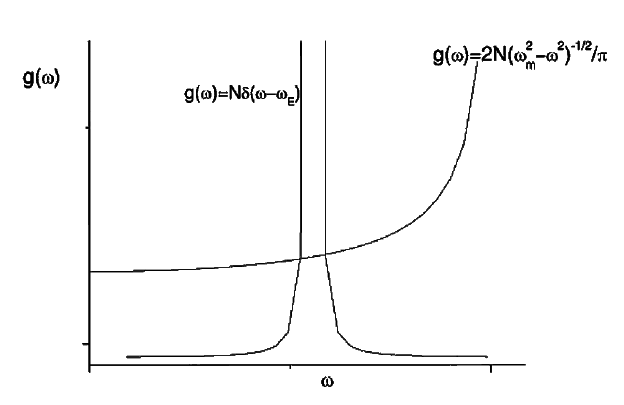
\includegraphics[width=0.5\textwidth]{pic/色散关系.png}
    \caption{色散关系}
    \label{fig:4.1}
\end{figure}

\noindent \textbf{4.\quad} 金刚石 (碳原子量为 $12$) 的杨氏模量为 \qty{e12}{N.m^{-2}},密度 $\rho=\qty{3.5}{g.cm^{-3}}$ 。试估算它的德拜温度 $\Theta_D=$?

\noindent \textbf{解:}

德拜温度为

\begin{equation*}
    \Theta_D = \frac{\hbar \omega_D}{k_B}
\end{equation*}

我们有

\begin{equation*}
    \omega_D = \left(\frac{6 \pi^2 N}{V}\right)^{\frac{1}{3}} V_s, \quad V_s = \sqrt{\frac{Y}{\rho}}
\end{equation*}

所以可得

\begin{align*}
    \Theta_D &= \frac{\hbar}{k_B} \sqrt{\frac{Y}{\rho}} \cdot \left(\frac{6 \pi^2 N}{V}\right)^{\frac{1}{3}} \\
    &= \frac{\hbar}{k_B} \sqrt{\frac{Y}{\rho}} \cdot \left(\frac{6 \pi^2 \rho}{M_C}\right)^{\frac{1}{3}} \\
    &= \frac{1.0546 \times 10^{-34}}{1.3807 \times 10^{-23}} \cdot \sqrt{\frac{10^{12}}{3.5 \times 10^3}} \left(\frac{6 \times 3.14^2 \times 3.5 \times 10^3}{12 \times 1.6605 \times 10^{-27}}\right)^{\frac{1}{3}} \unit{K} \\
    &\approx \qty{2817}{K} 
\end{align*}

\noindent \textbf{5.\quad} 试用德拜模型求晶体中各声频支格波的零点振动能。

\noindent \textbf{解:}

在德拜模型中,纵波与横波的最大振动频率均为 $\left(\frac{6 \pi^2 N}{V}\right)^{\frac{1}{3}} V_s$,其中 $\frac{1}{V_s^3}=\frac{1}{3} \left(\frac{1}{V_l^3}+\frac{2}{V_t^3}\right)$

\begin{equation*}
    g_l(\omega) = \frac{V}{2 \pi^2} \frac{\omega^2}{V_l^3}, \quad g_t(\omega) = \frac{V}{2 \pi^2} \frac{\omega^2}{V_t^3}
\end{equation*}

纵波的零点振动能为

\begin{align*}
    U_{0l} &= \int_0^{\omega_D} \frac{\hbar\omega}{2} \cdot g_l(\omega) \dif\omega \\
    &= \int_0^{\omega_D} \frac{\hbar\omega}{2} \cdot \frac{V}{2\pi^2} \frac{\omega^2}{V_l^3} \dif\omega \\
    &= \frac{\hbar V}{16 \pi^2 V_l^3} \omega_D^4
\end{align*}

同理可得,两支横波的零点振动能均为

\begin{align*}
    U_{0t} &= \int_0^{\omega_D} \frac{\hbar\omega}{2} \cdot g_t(\omega) \dif\omega \\
    &= \int_0^{\omega_D} \frac{\hbar\omega}{2} \cdot \frac{V}{2\pi^2} \frac{\omega^2}{V_t^3} \dif\omega \\
    &= \frac{\hbar V}{16 \pi^2 V_t^3} \omega_D^4
\end{align*}

故,总的零点振动能为

\begin{align*}
    U_0 &= U_{0l} + 2 U_{0t} \\
    &= \frac{\hbar V}{16 \pi^2 V_l^3} \omega_D^4 + 2 \frac{\hbar V}{16 \pi^2 V_t^3} \omega_D^4 \\
    &= \frac{3\hbar V}{16 \pi^2} \cdot \frac{1}{3} \left(\frac{1}{V_l^3}+\frac{2}{V_l^3}\right) \cdot \frac{6\pi^2 N}{V} V_s^3 \cdot \omega_D \\
    &= \frac{9N}{8} \hbar \omega_D
\end{align*}

\noindent \textbf{6.\quad} 一根直径为 \qty{3}{mm} 的人造蓝宝石晶体的热导率,在 \qty{30}{K} 的温度达到一个锐的极大值,试估计此极大值。(蓝宝石在 $T \ll \Theta_D = \qty{1000}{K}$ 时,$c_V=10^{-1} T^3 \unit{J.m^{-3}.K^{-1}}$)

\noindent \textbf{解:}

在低温情况下,热导率的表达式为

\begin{equation*}
    \kappa = \frac{1}{3} c_V v l
\end{equation*}

其中,$c_V=10^{-1} T^3 \unit{J.m^{-3}.K^{-1}}$, 而且由于直径很小,自由程 $l\approx d=\qty{3}{mm}$,所以

\begin{equation*}
    \kappa = 2.7 v
\end{equation*}

而声速 $v$ 由德拜模型求取,在德拜模型中,($N$为原胞个数)

\begin{equation*}
    \omega_D = \left(\frac{30\pi^2 N}{V}\right)^{\frac{1}{3}} V_s = \left(\frac{30 \pi^2 N \cdot M_{\ce{Al2O3}}}{V \cdot M_{\ce{Al2O3}}}\right)^{\frac{1}{3}} V_s, \quad \omega_D = \frac{\Theta_D k_B}{\hbar}
\end{equation*}

故,

\begin{equation*}
    V_s = \frac{\Theta_D k_s}{\hbar} \left(\frac{30 \pi^2 \rho}{M_{\ce{Al2O3}}}\right)^{-\frac{1}{3}} \approx \qty{6.84e3}{m.s^{-1}}
\end{equation*}

其中 $\rho=\qty{4}{g.cm^{-3}}$。

\begin{equation*}
    v = V_s \approx \qty{6.84e3}{m.s^{-1}}
\end{equation*}

代入 $\kappa=2.7 v$ 中,可得

\begin{equation*}
    \kappa = \qty{1.85e4}{W.m^{-1}.K^{-1}}
\end{equation*}

\noindent \textbf{7.\quad} \ce{Na} 和 \ce{Cl} 的原子量分别为 $23$ 和 $37$。氯化钠立方晶胞边长为 \qty{0.56}{nm},在 $[100]$ 方向可以看作是一组平行的离子链。离子间距 $d=\qty{0.28}{nm}$。\ce{NaCl} 晶体的杨氏模量为 \qty{5e10}{N.m^{-2}} 气如果全放射的光频率与 $q=0$ 的光频模频率相等,求对应的光波波长 (实验值为 \qty{61}{um}) 。

\noindent \textbf{解:}

在一维双原子链模型中,$q=0$ 时,光频模频率为

\begin{equation*}
    \omega(0) = \left[2\beta \left(\frac{1}{M_1}+\frac{1}{M_2}\right) \right]^{\frac{1}{2}}
\end{equation*}

杨氏模量为

\begin{equation*}
    Y = \frac{L}{A} \left(\frac{\partial F}{\partial l}\right)_T = \frac{d}{d^2} \beta
\end{equation*}

所以

\begin{equation*}
    \beta = dY
\end{equation*}

光波波长为

\begin{align*}
    \lambda &= cT = c \cdot \frac{2\pi}{\omega} \\
    &= \frac{2\pi c}{\left[2\beta \left(\frac{1}{M_1}+\frac{1}{M_2}\right)\right]^{\frac{1}{2}}} \\
    &= \frac{2\pi c}{\left[2dY \left(\frac{1}{M_1}+\frac{1}{M_2}\right)\right]^{\frac{1}{2}}} \\
    &\approx \qty{54.6}{um}
\end{align*}

\noindent \textbf{8.\quad} 立方晶体有三个弹性模量 $C_{11}, C_{12}$ 和 $C_{44}$。铝的 $C_{11}=\qty{10.82e10}{N.m^{-2}}, C_{44}=\qty{2.85e10}{N.m^{-2}}$,铝沿 $[100]$ 方向传播的弹性纵波的速度 $v_l=\sqrt{\frac{C_{11}}{\rho}}$,横波速度 $v_t=\sqrt{\frac{C_{44}}{\rho}}$,\ce{Al} 的密度 $\rho=\qty{2.70e3}{kg.m^{-3}}$ 气求德拜模型中铝的振动模式密度 $g(m)$。

\noindent \textbf{解:}

德拜模型中,振动模式密度为

\begin{equation*}
    g(\omega) = \frac{3V}{2\pi^2} \frac{\omega^2}{V_s^3}, \quad (\omega \le \omega_D)
\end{equation*}

其中

\begin{equation*}
    \omega_D = \left(\frac{6\pi^2 N}{V}\right)^{\frac{1}{3}} V_s, \quad \frac{1}{V_s^3} = \frac{1}{3} \left(\frac{1}{V_l^3}+\frac{2}{V_t^3}\right)
\end{equation*}

将 $v_l=\sqrt{\frac{C_{11}}{\rho}}, v_t=\sqrt{\frac{C_{44}}{\rho}}$ 代入上式可得

\begin{align*}
    \frac{1}{V_s^3} &= \frac{1}{3} \left(\frac{1}{V_l^3}+\frac{2}{V_t^3}\right) \\
    &= \frac{1}{3} \left[\left(\frac{\rho}{C_{11}}\right)^{\frac{3}{2}}+2\left(\frac{\rho}{C_{44}}\right)^{\frac{3}{2}}\right] \\
    &\approx \qty{2.075e-11}{m^{-3}.s^3}
\end{align*}

所以

\begin{equation*}
    V_s = \qty{3.64e3}{m·s^{-1}}
\end{equation*}

代入 $\omega_D$ 中,

\begin{align*}
    \omega_D &= \left(\frac{6\pi^2 N}{V}\right)^{\frac{1}{3}} V_s \\
    &= \left(\frac{6\pi^2 N \cdot M_{\ce{Al}}}{V \cdot M_{\ce{Al}}}\right)^{\frac{1}{3}} V_s \\
    &= \left(\frac{6\pi^2 \rho}{M_{\ce{Al}}}\right)^{\frac{1}{3}} V_s \\
    &\approx \qty{5.56e13}{rad.s^{-1}}
\end{align*}

所以

\begin{align*}
    g(\omega) &= \frac{3V}{2\pi^2} \frac{\omega^2}{V_s^3} \\
    &= \frac{3}{2 \times 3014^2} \times 2.075 \times 10^{-12} \omega^2 V \\
    &\approx 3.157 \times 10^{-12} \omega^2 V
\end{align*}

其中

\begin{equation*}
    \omega \le \omega_D = \qty{5.56e13}{rad.s^{-1}}
\end{equation*}

\chapter{\label{ch:5}}

没有习题解答。

\chapter{金属电子论\label{ch:6}}

\noindent \textbf{1.\quad}导出一维和二维自由电子气的能态密度。

\noindent \textbf{解:}

一维情形:

自由电子的 Schrödinger 方程为

\begin{equation*}
    -\frac{\hbar^2}{2m} \cdot \frac{\dif^2 \varphi}{\dif x^2} = E \varphi
\end{equation*}

自由电子波函数的解为

\begin{equation*}
    \dif Z = 2 \cdot \frac{L}{2\pi} \cdot 2 \dif k = \frac{2L}{\pi} \dif k = \frac{2L}{\pi} \frac{\sqrt{2m}}{\hbar} \frac{\dif E}{2 \sqrt{E}} = \frac{L}{\pi} \frac{\sqrt{2m}}{\hbar} \frac{\dif E}{\sqrt{E}}
\end{equation*}

且有

\begin{equation*}
    E = \frac{\hbar^2 k^2}{2m}
\end{equation*}

由周期性边界条件 $\varphi(x+L)=\varphi(x)$ ,可得

\begin{equation*}
    k = \frac{2\pi}{L} n
\end{equation*}

在 $k=\sqrt{2mE}/\hbar$ 处于区间 $[k, k+\dif k]$ 时候

由于 $\dif Z = L g_1(E) \dif E$,对比可得

\begin{equation*}
    g_1(E) = \frac{\sqrt{2m}}{\pi\hbar} E^{-\frac{1}{2}}
\end{equation*}

二维情形:

同上,由电子的 Schrödinger 方程:

\begin{equation*}
    -\frac{\hbar^2}{2m} \nabla^2 \varphi = E \varphi
\end{equation*}

得自由电子波函数解:

\begin{equation*}
    \varphi(\mathbf{r}) = \frac{1}{\sqrt{S}} e^{i \mathbf{k} \cdot \mathbf{r}}, \quad S = L^2
\end{equation*}

且

\begin{equation*}
    E(\mathbf{k}) = \frac{\hbar^2 k^2}{2m} = \frac{hbar^2}{2m} (k_x^2 + k_y^2)
\end{equation*}

由周期性边界条件可得

\begin{equation*}
    \begin{cases}
        \varphi(x+L, y) = \varphi(x, y) \\
        \varphi(x, y+L) = \varphi(x, y)
    \end{cases}
\end{equation*}

可得

\begin{equation*}
    k_x = \frac{2\pi}{L} n_x, \quad k_y = \frac{2\pi}{L} n_y
\end{equation*}

在区间 $[k=\sqrt{2mE}/\hbar, k+\dif k]$ 内

\begin{equation*}
    \dif Z = 2 \cdot \frac{S}{(2\pi)^2} \dif \mathbf{k} = \frac{S}{2\pi^2} \cdot 2\pi k \dif k = \frac{mS}{\pi \hbar^2} \dif E
\end{equation*}

同理,与 $\dif Z=S g_2(E) \dif E$ 比较可得

\begin{equation*}
    g_2(E) = \frac{m}{\pi \hbar}
\end{equation*}

\noindent \textbf{2.\quad} 若二维电子气的面密度为 $n_s$,证明它的化学势为:

\begin{equation*}
    \mu = k_B T \ln \left[\exp\left(\frac{\pi\hbar^2 n_s}{m k_B T}\right)-1\right]
\end{equation*}

\noindent \textbf{解:}

由前一题已经求得能态密度

\begin{equation*}
    g(E) = \frac{m}{\pi\hbar}
\end{equation*}

电子气体的化学势 $\mu$ 由下式决定:

\begin{equation*}
    N = \int_0^\infty g(E) L^2 \dif E = \frac{L^2}{\pi \hbar^2} \int_0^\infty \frac{\dif E}{e^{(E-\mu)/k_B T}+1}
\end{equation*}

我们令 $x\equiv(E-\mu)/k_B T$,注意到 $n_s=\frac{N}{L^2}$

\begin{align*}
    n_s &= \frac{k_B T m}{\pi\hbar^2} \int_{-\mu/k_B T}^{\infty} \frac{1}{e^x+1} \dif x \\
    &= \frac{k_B T m}{\pi\hbar^2} \int_{-\mu/k_B T}^{\infty} \frac{\dif e^x}{e^x(e^x+1)} \\
    &= \frac{k_B T m}{\pi\hbar^2} \left. \ln\frac{e^x}{e^x+1} \right|_{-\mu/k_B T}^{\infty} \\
    &= \frac{k_B T m}{\pi\hbar^2} \ln \left(e^{\mu/k_B T}+1\right)
\end{align*}

那么可以求出 $\mu$

\begin{equation*}
    \mu = k_B T \ln \left[\exp\left(\frac{\pi\hbar^2 n_s}{m k_B T}\right)-1\right]
\end{equation*}

\noindent \textbf{3.\quad} \ce{^3 He} 是费米子,液体 \ce{^3 He} 在绝对零度附近的密度为 \qty{0.081}{g.cm^{-3}}。计算它的费米能压和费米温度 $T_F$。

\noindent \textbf{解:}

\ce{^3 He} 的数密度:

\begin{equation*}
    n = \frac{N}{V} = \frac{N}{M} \cdot \frac{M}{V} = \rho \cdot \frac{N}{M} = \frac{\rho}{m}
\end{equation*}

其中 $m$ 为单个 \ce{^3 He} 粒子的质量

\begin{equation*}
    k_F = (3\pi^2 n)^{\frac{1}{3}} = \left(\frac{6\pi^2 \rho}{m}\right)^{\frac{1}{3}}
\end{equation*}

可得

\begin{equation*}
    E_F = \frac{\hbar^2 k^2}{2m} = \frac{\hbar^2}{2m} \left(\frac{6\pi^2 \rho}{m}\right)^{\frac{2}{3}}
\end{equation*}

代入数据,可以算得:

\begin{equation*}
    E_F = \qty{6.8577e-23}{J} = \qty{4.28e-4}{eV}
\end{equation*}

则:

\begin{equation*}
    T_F = \frac{E_F}{k_B} = \qty{4.79}{K}
\end{equation*}

\noindent \textbf{4.\quad} 金属钾在低温下的摩尔电子比热的实验值为:$c_e= 2.08 T \unit{mJ/(mol.K)}$, 试用自由电子气模型求它的费米能扁及状态密度 $g(E_F)$

\noindent \textbf{解:}

考虑费米球模型,在费米面以内的粒子吸收能量跃出费米面的数目期望是:

\begin{equation*}
    \overline{N} = c \int_{E_F-\frac{3}{2}kT}^{\infty} E^{1/2} \dif E = \frac{9}{4} N \frac{kT}{E_F}
\end{equation*}

这些粒子共吸收能量:

\begin{equation*}
    \overline{E} = \frac{\overline{N} \cdot \frac{3}{2}kT}{N} = \frac{27}{4} \cdot \frac{k_B^2 T^2}{E_F}
\end{equation*}

则相应的热容量为:

\begin{equation*}
    C_{ve} = \frac{\partial \overline{E}}{\partial E} = \frac{27}{4} \cdot \frac{k_B^2 T}{E_F} = \lambda T
\end{equation*}

其中:$\lambda=\frac{27}{4} \cdot \frac{k_B^2}{E_F}$

由题设数据,代入上式,可求出 $E_F$ 及 $g(E_F)$:

\begin{align*}
    E_F &= \frac{27 k_B^2 N_A}{4} = \qty{2.235e-3}{eV} \\
    g(E_F) &= \frac{3n V_N}{2 E_F} = \frac{3 N_A}{2 E_F} = \num{2.425e45}
\end{align*}

\noindent \textbf{5.\quad} 银是一价金属,在 $T=\qty{295}{K}$ 时,银的电阻率 $P=\qty{1.61e-6}{\Omega.cm}$,在 $T=\qty{20}{K}$ 时,电阻率 $\rho=\qty{0.038e-9}{\Omega.cm}$。求在低温和室温时电子的自由程。银的原子量为 $107.87$,密度为 \qty{10.5}{g/cm^3}。

\noindent \textbf{解:}

由

\begin{equation*}
    \rho = \frac{1}{\sigma} = \frac{m V_F}{n e^2 l}
\end{equation*}

可得

\begin{equation*}
    l = \frac{m V_F}{n e^2 \rho}
\end{equation*}

又因为

\begin{equation*}
    n = \frac{N}{V} = \frac{N}{M} \frac{M}{V} = \rho_0 \cdot \frac{N}{N_A} \cdot \frac{N_A}{M} = \frac{\rho_0 \cdot N_A}{M_s}
\end{equation*}

其中 $N_A$ 为阿伏加德罗常数,$M_s$ 为 \ce{Ag} 的原子溢,$\rho_0$ 为 \ce{Ag} 的密度。将上式代入 $l$ 的表达式,并代入数据可得:

当 $T=\qty{295}{K}$ 时,$l=\qty{3.7e-4}{m}$,

当 $T=\qty{20}{K}$ 时,$l=\qty{1.6}{m}$,

在计算过程中,已取 $V_F=\qty{e6}{m}$。

\noindent \textbf{6.\quad} Hunter S.C 和 F.R.N.Nabarro 曾计算铜中每厘米位错线引起的电阻率如下:

\begin{enumerate}
    \item 刃型位错 $\Delta_{\rho E} = \qty{0.59e-20}{\Omega.cm}$
    \item 螺型位错 $\Delta_{\rho s} = \qty{0.18e-20}{\Omega.cm}$
\end{enumerate}

假定刃型位错和螺型位错有相同的密度 (位错密度为 \qty{1}{cm^2} 有多少条位错线)。已知位错产生的电阻率 $\Delta \rho = \qty{2e-8}{\Omega.cm}$,问铜中的位错密度是多少?

\noindent \textbf{解:}

设密度为 $X$,由题意可以列出方程:

\begin{equation*}
    \left(\Delta_{\rho E} + \Delta_{\rho E}\right) \cdot x = \Delta \rho
\end{equation*}

\noindent \textbf{7.\quad} 在室温下金属铍的霍尔系数为 \qty{2.44e-10}{m^3.C^{-1}},求铍中空穴密度。

\noindent \textbf{解:}

由霍尔系数定义 $R_H=\frac{1}{pe}$ 得

\begin{equation*}
    p = \frac{1}{e \cdot R_H} = \qty{2.56e28}{m^{-3}}
\end{equation*}

\noindent \textbf{8.\quad} 试计算 \ce{Cs} 在 $T=\qty{1000}{K}$ 时热电子发射的电流密度。

\noindent \textbf{解:}

电子热发射的电流密度函数为:

\begin{equation*}
    j = 4\pi e \left[\frac{m(kT)^2}{\hbar^3}\right] e^{-\frac{\phi}{kT}}
\end{equation*}

查表可得 \ce{Cs} 的功函数为 \qty{1.81}{eV}。代入数据到上式中可以算得:

\begin{equation*}
    j = \qty{9.2e2}{A.m^{-2}}
\end{equation*}

\noindent \textbf{9.\quad} \ce{Al} 等离子体能量 $\hbar \omega_p$ 的实验值为 \qty{15.3}{eV},按照自由电子气模型的电子密度为 $n=\qty{18.06e22}{m^{-3}}$, 求 $\hbar \omega_p$ 的理论值。

\noindent \textbf{解:}

由等离子体振荡频率关系式:

\begin{equation*}
    \omega_p^2 = \frac{n e^2}{\varepsilon_0 m}
\end{equation*}

故:

\begin{equation*}
    \hbar \omega_p = \hbar e \sqrt{\frac{n}{\varepsilon_0 m}} = \qty{15.7}{eV}
\end{equation*}

\chapter{周期场中的电子态\label{ch:7}}

\noindent \textbf{1.\quad} 一维周期场中电子的波函数 $\psi_k(x)$ 应满足布洛赫定理。若晶体常数是 $a$,电子的波函数为

\begin{align*}
    (1) \quad & \Psi_k(x) = \sin \frac{\pi}{a}x \\
    (2) \quad & \Psi_k(x) = i \cos \frac{3\pi}{a}x \\
    (3) \quad & \Psi_k(x) = \sum_{l=-\infty}^{\infty} f(x-la)
\end{align*}

试求电子在这些状态的波矢。

\noindent \textbf{解:}

\begin{equation*}
    T_l \Psi = e^{i \vec{k} \cdot \vec{R}_l} \Psi
\end{equation*}

\begin{equation*}
    (1) \quad \Psi_k(x+a) = \sin \frac{\pi}{a} (x+a) = e^{i\pi} \Psi_k(x) = e^{ika} \Psi_k (x)
\end{equation*}

\begin{equation*}
    \therefore ka = \pi, \quad k = \frac{\pi}{a}
\end{equation*}

\begin{equation*}
    (2) \quad \Psi_k(x+a) = i\cos \frac{3\pi}{a} (x+a) = e^{i\pi} \Psi_k(x) = e^{ika} \Psi_k (x)
\end{equation*}

\begin{equation*}
    \therefore ka = \pi, \quad k = \frac{\pi}{a}
\end{equation*}

\begin{equation*}
    (3) \quad \Psi_k(x+a) = \sum_{l=-\infty}^{\infty} f(x+a-la) = \sum_{l=-\infty}^{\infty} f[x-(l-1)a] = \sum_{l=-\infty}^{\infty} f(x-la) \Psi_k (x)
\end{equation*}

\begin{equation*}
    \therefore ka = 0, \quad k = 0
\end{equation*}

\noindent \textbf{2.\quad} 电子在周期场中的势能

\begin{equation*}
    V(x) =
    \begin{cases}
        \frac{1}{2} m \omega^2 \left[b^2-(x-na)^2\right] & na-b \le x \le na+b \\
        0 & (n-1)a+b \le x \le na-b
    \end{cases}
\end{equation*}

且 $a=4b$,$\omega$ 是常数。试画出此势能曲线,并求此势能的平均值。

\noindent \textbf{解:}

势能曲线为:

\begin{equation*}
    \overline{V} = \frac{1}{a} \int_{-\frac{a}{4}}^{\frac{a}{4}} V(x) \dif x = \frac{1}{a} \int_{-\frac{a}{4}}^{\frac{a}{4}} \frac{1}{2} m \omega^2 \left[b^2 - (x-na)^2\right] \dif x = \frac{m \omega^2 a^2}{96}
\end{equation*}

\noindent \textbf{3.\quad} 用近自由电子模型处理上题,并求此晶体的第一个以及第二个禁带宽度。

\noindent \textbf{解:}

\begin{equation*}
    V(x) = \sum_n V_n e^{in \frac{2\pi}{a} x} = V_0 + \sum_{n \ne 0} V_n e^{in \frac{2\pi}{a} x}
\end{equation*}

为简单计算,令 $V_0=0$

\begin{align*}
    V_1 = \frac{1}{a} \int_{-\frac{a}{2}}^{\frac{a}{2}} V(x) e^{-i \frac{2\pi}{a} x} \dif x = \frac{m \omega^2 a^2}{4 \pi^2} \\
    V_2 = \frac{1}{a} \int_{-\frac{a}{2}}^{\frac{a}{2}} V(x) e^{-i \frac{4\pi}{a} x} \dif x = \frac{m \omega^2 a^2}{32 \pi^2}
\end{align*}

计算表明,第一个禁带宽度为:

\begin{equation*}
    2|V_1| = \frac{m \omega^2 a^2}{2\pi^2}
\end{equation*}

第二个禁带宽度为:

\begin{equation*}
    2|V_2| = \frac{m \omega^2 a^2}{16\pi^2}
\end{equation*}

\noindent \textbf{4.\quad} 已知一维晶体的电子能带可写成

\begin{equation*}
    E(k) = \frac{\hbar^2}{m a^2} \left(\frac{7}{8}-\cos ka + \frac{1}{8} \cos 2ka\right)
\end{equation*}

式中 $a$ 是晶格常数。试求:

\begin{enumerate}
    \item 能带的宽度;
    \item 电子在波矢 $k$ 的状态时的速度;
    \item 能带底部和顶部电子的有效质量。
\end{enumerate}

\noindent \textbf{解:}

\begin{enumerate}
    \item 分析能量的表达式
        \begin{align*}
            E(k) &= \frac{\hbar^2}{m a^2} \left(\frac{7}{8}-\cos{ka} + \frac{1}{8} \cos 2ka\right) \\
            &= \frac{\hbar^2}{m a^2} \left[\frac{1}{4} \left(\cos{ka}-2\right)^2 - \frac{1}{4}\right] \\
        \end{align*}
        当 $k=0$ 时,$E_{min}=0$;当 $k=\frac{\pi}{a}$ 时,$E_{max}=\frac{2\hbar^2}{m a^2}$。所以能带的宽度为
        \begin{equation*}
            \Delta E = E_{max} - E_{min} = \frac{2\hbar^2}{m a^2}
        \end{equation*}
    \item 电子的速度为
        \begin{align*}
            \vec{v} &= \frac{1}{\hbar} \Delta_k E(\vec{k}) \\
            &= -\frac{\hbar}{4ma} (\sin{2ka} - 4 \sin{ka})
        \end{align*}
    \item 能带底部,将 $E(k)$ 在 $k=0$ 附近用泰勒展开,可得
        \begin{equation*}
            E = E_{min} + \frac{\hbar^2 k^2}{4m} = E_{min} + \frac{\hbar^2 k^2}{2 m^*}
        \end{equation*}
        比较可得
        \begin{equation*}
            m^* = 2m
        \end{equation*}
        同理,在能带顶部,将 $E(k)$ 在 $k=\frac{\pi}{a}$ 附近用泰勒展开,令 $k=\frac{\pi}{a}+\delta k$,可得
        \begin{equation*}
            E = E_{max} - \frac{3\hbar^2}{4m} (\delta k)^2 = E_{max} + \frac{\hbar^2 (\delta k)^2}{2 m^*}
        \end{equation*}
        比较可得
        \begin{equation*}
            m^* = -\frac{2}{3} m < 0
        \end{equation*}
\end{enumerate}

\noindent \textbf{5.\quad} 如图所示平面正六方晶格是复式格子,若原胞中的原子属千同一元素,试求此晶体的结构因子。

\noindent \textbf{解:}

如图所示:由于红色和紫色的原子不等价,阴影部分为一个原胞。原胞中包含两个原子。

\begin{figure}[htbp]
    \centering
    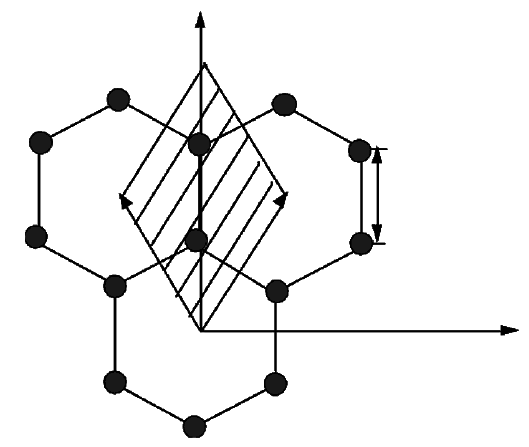
\includegraphics[width=0.5\textwidth]{pic/六方复式格子.png}
    \caption{六方复式格子}
    \label{fig:7.1}
\end{figure}

设 $\vec{a}_3=\vec{k}$,由图可得:

\begin{equation*}
    \vec{a}_1 = \frac{\sqrt{3}}{2} a \vec{i} + \frac{3}{2} a \vec{j}, \quad \vec{a}_2 = -\frac{\sqrt{3}}{2} a \vec{i} + \frac{3}{2} a \vec{j}
\end{equation*}

则原胞面积

\begin{equation*}
    A_c = \Omega = \vec{a}_3 \cdot (\vec{a}_1 \times\vec{a}_2) = \frac{3\sqrt{3}}{2} a^2
\end{equation*}

\begin{align*}
    \vec{b}_1 &= \frac{2\pi (\vec{a}_2 \times \vec{a}_3)}{\Omega} = \frac{2\pi}{a} \left(\frac{\sqrt{3}}{3}\vec{i} + \frac{1}{3}\vec{j}\right) \\
    \vec{b}_2 &= \frac{2\pi (\vec{a}_3 \times \vec{a}_1)}{\Omega} = \frac{2\pi}{a} \left(-\frac{\sqrt{3}}{3}\vec{i} + \frac{1}{3}\vec{j}\right) \\
    \vec{k}_h = \vec{b}_1 + \vec{b}_2 = \frac{4\pi}{3a} \vec{j}
\end{align*}

原胞中两个原子相对于原胞顶点的位矢分别为:

\begin{align*}
    \vec{d}_1 &= \frac{1}{3} \vec{a}_1 + \frac{1}{3} \vec{a}_2 = a \vec{j} \\
    \vec{d}_2 &= \frac{2}{3} \vec{a}_1 + \frac{2}{3} \vec{a}_2 = 2a \vec{j}
\end{align*}

晶体的结构因子为

\begin{equation*}
    S(\vec{k}_h) = \sum_{j=1}^{2} e^{-i \vec{k}_h \cdot \vec{d}_j} = e^{-i \frac{4\pi}{3a}\vec{j} \cdot a\vec{j}} + e^{-i \frac{4\pi}{3a}\vec{j} \cdot 2a\vec{j}} = -1
\end{equation*}

\noindent \textbf{6.\quad} 用紧束缚方法处理面心立方晶体的 $s$ 态电子,若只计最近邻的相互作用,试导出其能带为:

\begin{equation*}
    E(\vec{k}) = E_0 - A - 4J \left[\cos{\frac{k_x a}{2}}\cos{\frac{k_y a}{2}} + \cos{\frac{k_y a}{2}}\cos{\frac{k_z a}{2}} + \cos{\frac{k_z a}{2}}\cos{\frac{k_x a}{2}}\right]
\end{equation*}

并求能带底部电子的有效质量。

\noindent \textbf{解:}

面心立方的每个格点有 $12$ 个最近邻,如晶格常数为 $a$,取某格点为坐标原点,则这 $12$ 个最近邻的坐标为:

\begin{equation*}
    \begin{matrix}
        (\frac{a}{2}, -\frac{a}{2}, 0) & (\frac{a}{2}, \frac{a}{2}, 0) & (-\frac{a}{2}, \frac{a}{2}, 0) & (-\frac{a}{2}, -\frac{a}{2}, 0) \\
        (0, -\frac{a}{2}, -\frac{a}{2}) & (0, \frac{a}{2}, -\frac{a}{2}) & (0, \frac{a}{2}, \frac{a}{2}) & (0, -\frac{a}{2}, \frac{a}{2}) \\
        (\frac{a}{2}, 0, -\frac{a}{2}) & (\frac{a}{2}, 0, \frac{a}{2}) & (-\frac{a}{2}, 0, \frac{a}{2}) & (-\frac{a}{2}, 0, -\frac{a}{2})
    \end{matrix}
\end{equation*}

\begin{align*}
    E(\vec{k}) &= E^s + C - J \bigg[e^{i\vec{k}\cdot\left(\frac{a}{2}\vec{i}-\frac{a}{2}\vec{j}\right)} + e^{i\vec{k}\cdot\left(\frac{a}{2}\vec{i}+\frac{a}{2}\vec{j}\right)} + e^{i\vec{k}\cdot\left(-\frac{a}{2}\vec{i}+\frac{a}{2}\vec{j}\right)} + e^{i\vec{k}\cdot\left(-\frac{a}{2}\vec{i}-\frac{a}{2}\vec{j}\right)} \\
    &\quad\quad\quad\quad\quad\quad\quad e^{i\vec{k}\cdot\left(\frac{a}{2}\vec{j}-\frac{a}{2}\vec{k}\right)} + e^{i\vec{k}\cdot\left(\frac{a}{2}\vec{j}+\frac{a}{2}\vec{k}\right)} + e^{i\vec{k}\cdot\left(-\frac{a}{2}\vec{j}+\frac{a}{2}\vec{k}\right)} + e^{i\vec{k}\cdot\left(-\frac{a}{2}\vec{i}-\frac{a}{2}\vec{j}\right)} \\
    &\quad\quad\quad\quad\quad\quad\quad e^{i\vec{k}\cdot\left(\frac{a}{2}\vec{i}-\frac{a}{2}\vec{k}\right)} + e^{i\vec{k}\cdot\left(\frac{a}{2}\vec{i}+\frac{a}{2}\vec{k}\right)} + e^{i\vec{k}\cdot\left(-\frac{a}{2}\vec{i}+\frac{a}{2}\vec{k}\right)} + e^{i\vec{k}\cdot\left(-\frac{a}{2}\vec{i}-\frac{a}{2}\vec{k}\right)}\bigg] \\
    &= E^s + C - 4J \left[\cos{\frac{k_x a}{2}}\cos{\frac{k_y a}{2}} + \cos{\frac{k_y a}{2}}\cos{\frac{k_z a}{2}} + \cos{\frac{k_z a}{2}}\cos{\frac{k_x a}{2}}\right]
\end{align*}

对于上式表示的能带,其最小值位于倒空间的原点

\begin{equation*}
    E_{min} = E^s + C - 12J
\end{equation*}

令 $E_0 = E_{min}, A=-12J$,则有

\begin{equation*}
    E(\vec{k}) = E_0 - A - 4J \left[\cos{\frac{k_x a}{2}}\cos{\frac{k_y a}{2}} + \cos{\frac{k_y a}{2}}\cos{\frac{k_z a}{2}} + \cos{\frac{k_z a}{2}}\cos{\frac{k_x a}{2}}\right]
\end{equation*}

将上式中三角函数在 $k=0$ 附近展开,可得:

\begin{align*}
    E(\vec{k}) &= E_{min} + J a^2 (k_x^2+k_y^2+k_z^2) \\
    &= E_{min} + \frac{\hbar^2 k^2}{2 m^*}
\end{align*}

比较可得

\begin{equation*}
    m^* = \frac{\hbar^2}{2J a^2} > 0
\end{equation*}

\noindent \textbf{7.\quad} 二维正方晶格的周期性势场可表示为:

\begin{equation*}
    V(x, y) = -4U \cos\left(\frac{2\pi}{a}x\right) \cos\left(\frac{2\pi}{a}y\right)
\end{equation*}

$a$ 为晶格常数,试由自由电子近似计算布里渊区边界点 $(\frac{\pi}{a}, \frac{\pi}{a})$ 处的能隙。

\noindent \textbf{解:}

\begin{align*}
    V(x, y) &= \sum_{m, n} V_{mn} e^{im\frac{2\pi}{a}x} e^{in\frac{2\pi}{a}y} \\
    &= V_{00} + \sum_{m\ne 0, n\ne 0} V_{mn} e^{im\frac{2\pi}{a}x} e^{in\frac{2\pi}{a}y} \\
\end{align*}

为简单计算,令 $V_{00}=0$

\begin{equation*}
    V_{mn} = \frac{1}{a^2} \int_{-\frac{a}{2}}^{\frac{a}{2}} \int_{-\frac{a}{2}}^{\frac{a}{2}} V(x, y) e^{-im\frac{2\pi}{a}x} e^{-in\frac{2\pi}{a}y} \dif x \dif y
\end{equation*}

在边界点 $\left(\frac{\pi}{a}, \frac{\pi}{a}\right)$ 处,$m=n=1$

\begin{align*}
    V_{11} &= \frac{1}{a^2} \int_{-\frac{a}{2}}^{\frac{a}{2}} \int_{-\frac{a}{2}}^{\frac{a}{2}} V(x, y) e^{-i\frac{2\pi}{a}x} e^{-i\frac{2\pi}{a}y} \dif x \dif y \\
    &= \frac{1}{a^2} \int_{-\frac{a}{2}}^{\frac{a}{2}} \int_{-\frac{a}{2}}^{\frac{a}{2}} V(x, y) \cos{\frac{2\pi}{a}x} \cos{\frac{2\pi}{a}y} \dif x \dif y \\
    &= \frac{-4U}{a^2} \left[\int_{-\frac{a}{2}}^{\frac{a}{2}} \cos^2{\frac{2\pi}{a}x}\right]^2 \\
    &= \frac{-4U}{a^2} \left(\frac{a}{2}\right)^2 \\
    &= -U
\end{align*}

所以,在边界点 $\left(\frac{\pi}{a}, \frac{\pi}{a}\right)$ 处的能隙为

\begin{equation*}
    2|V_{11}| = 2U
\end{equation*}

\noindent \textbf{8.\quad} 图为二维正三角形晶格,相邻原子间距为 $a$, 只计入最近邻相互作用,试用紧束缚近似计算其 $s$ 电子能带 $\Delta E$、带中电子的速度 $v(k)$ 以及能带极值附近的有效质量 $m^*$。

\begin{figure}[htbp]
    \centering
    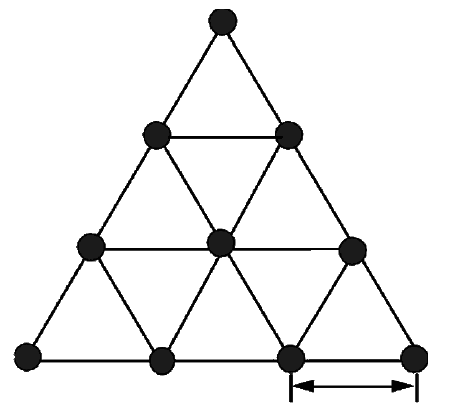
\includegraphics{pic/二维正三角晶格.png}
    \caption{二维正三角晶格}
    \label{fig:7.2}
\end{figure}

\noindent \textbf{解:}

三角形晶格的每个格点有 $6$ 个最近邻,晶格常数为 $a$,取某格点为坐标原点,则这 $6$ 个最近邻的坐标为:

\begin{equation*}
    (a, 0), \quad (\frac{a}{2}, \frac{\sqrt{3}}{2}a), \quad (-\frac{a}{2}, \frac{\sqrt{3}}{2}a), \quad (-a, 0), \quad (-\frac{a}{2}, \frac{\sqrt{3}}{2}a), \quad (\frac{a}{2}, -\frac{\sqrt{3}}{2}a)
\end{equation*}

\begin{align*}
    E(\vec{k}) &= E^s + C - J \sum_l e^{i\vec{k}\cdot\vec{R}_l} \\
    &= E^s + C - J \left[e^{i\vec{k}\cdot a\vec{i}} + e^{i\vec{k}\cdot \left(\frac{a}{2}\vec{i}+\frac{\sqrt{3}}{2}a\vec{j}\right)} + e^{i\vec{k}\cdot \left(-\frac{a}{2}\vec{i}+\frac{\sqrt{3}}{2}a\vec{j}\right)} + e^{i\vec{k}\cdot (-a\vec{i})} + e^{i\vec{k}\cdot \left(-\frac{a}{2}\vec{i}-\frac{\sqrt{3}}{2}a\vec{j}\right)} + e^{i\vec{k}\cdot \left(\frac{a}{2}\vec{i}-\frac{\sqrt{3}}{2}a\vec{j}\right)}\right] e^{i\vec{k}\cdot\vec{R}_l} \\
    &= E^s + C - J \left(2\cos{k_x a} + 4\cos{\frac{k_x a}{2}} \cos{\frac{\sqrt{3}k_y a}{2}}\right)
\end{align*}

\begin{align*}
    E(\vec{k}) &= \frac{1}{\hbar} \Delta_k(\vec{k}) \\
    &= \frac{2Ja}{\hbar} \left[\left(\sin{k_x a} + \sin{\frac{k_x a}{2}} \cos{\frac{\sqrt{3}k_y a}{2}}\right) \vec{e}_x + \left(\sqrt{3} \cos{\frac{k_x a}{2}} \sin{\frac{\sqrt{3}k_y a}{2}}\right) \vec{e}_y\right]
\end{align*}

倒空间的原点 $(0, 0)$ 处,能带的极小值为

\begin{equation*}
    E_{min} = E^s + C - 6J
\end{equation*}

倒空间 $(\frac{4\pi}{3a}, 0)$ 或 $(\frac{2\pi}{3a}, \frac{2\pi}{\sqrt{3}a})$ 处,能带的极大值为

\begin{equation*}
    E_{max} = E^s + C + 3J
\end{equation*}

所以能带大小为

\begin{equation*}
    \Delta E = 9J
\end{equation*}

在能带极小值,将 $E(\vec{k})$ 中的三角函数在 $\vec{k}=0$ 附近用泰勒级数展开可得:

\begin{equation*}
    E(\vec{k}) = E_{min} + \frac{3}{2} J a^2 (k_x^2 + k_y^2) = E_{min} + \frac{\hbar^2 k^2}{2 m^*}
\end{equation*}

比较可得

\begin{equation*}
    m^* = \frac{\hbar^2}{3J a^2}
\end{equation*}

在能带极大值,如 $(\frac{4\pi}{3a}, 0)$ 附近将 $E(\vec{k})$ 中的三角函数用泰勒级数展开,令 $k_x=\frac{4\pi}{3a}+\delta k_x, k_y=\delta k_y$,可得

\begin{equation*}
    E(\vec{k}) = E_{max} - \frac{3}{4}J a^2 \left[(\delta k_x)^2 + (\delta k_y)^2\right] = E_{min} + \frac{\hbar2 (\delta k)^2}{2 m^*}
\end{equation*}

比较可得

\begin{equation*}
    m^* = -\frac{2\hbar^2}{3J a^2} < 0
\end{equation*}



\appendix
% \include{pages/appendix}
% \include{pages/appendix}


\backmatter
% \include{epilogue} % 后记epilogue.tex
% \bibliography{reference}
\printindex % 利用 makeindex 工具生成索引

\end{document}